%!TEX root = ../USthesis_Masters.tex

\chapter{Literature Study}
\label{chp:literature_study}



%%%%%%%%%%%%%%%%%%%%%%%%%%%%%%%%%%%%%%%%%%%%%%%%%%%%%%%%%%%%%%%%%%%%%%%
\section{Bitcoin}

Bitcoin is a protocol that was introduced in 2008\cite{Nakamoto2008}. Bitcoin is a digital currency that allows a user to send money in the form of Bitcoin to any other Bitcoin address in the world. The transactions are verified by the Bitcoin network - a peer-to-peer network of computers or Bitcoin nodes that independently run Bitcoin software. 

Bitcoin is decentralised which means that no country, organization or person controls it. It uses cryptography to remove trust from a central authority. With other payment mechanisms, a trusted third party is required to prevent double-spending \cite{Nakamoto2008}. Double-spending is a problem in digital payment systems that allows a malicious user to spend the same money twice. Bitcoin solves the double-spending problem by using a proof-of-work chain that can be trusted as long as the majority of the Bitcoin network is controlled by honest nodes.

The code that is responsible for the Bitcoin network is open source and is maintained by a core team of developers. Since the code is open source, anyone can verify the code to ensure it is not malicious. Each node on the network chooses what code to run, but nodes must reach consensus by means of the majority of the network accepting or rejecting certain transactions.



\subsection{A Bitcoin Address}

A Bitcoin address is similar to a bank account that people can pay money to. An address is an alphanumeric string, like \\1EZzmuCJqb6yhiowbdd7qgBQsiAJS4YEn3, that is used as a destination for a payment. An address is only an identifier of the wallet that it belongs to, and cannot be used to spend the Bitcoin that belongs to it. 

A Bitcoin address has two parts, a private key and a public key. The private key is an unsigned 256 bit integer that is usually randomly generated, but can also be chosen by the user. This private key should be kept secret, as anyone with the key can spend any Bitcoin that belongs to it.

The public key is generated from the private key using the Elliptic Curve Digital Signature Algorithm\cite{Johnson2001} with parameters specified in the secp256k1 specification \cite{bwSecp}\cite{Research2010} that was chosen for the Bitcoin protocol. The public address is generated from the public key with a series of hashes shown in figure \ref{fig:PubKeyToAddr}. This allows the public key to only be made public once funds from an address are spent and not when receiving funds. This adds a layer of security to reduce risk.

\begin{figure}
  \centering
  	\caption{Public Key To Address Conversion. Adapted from \cite{pubkeytoadd}.} 
    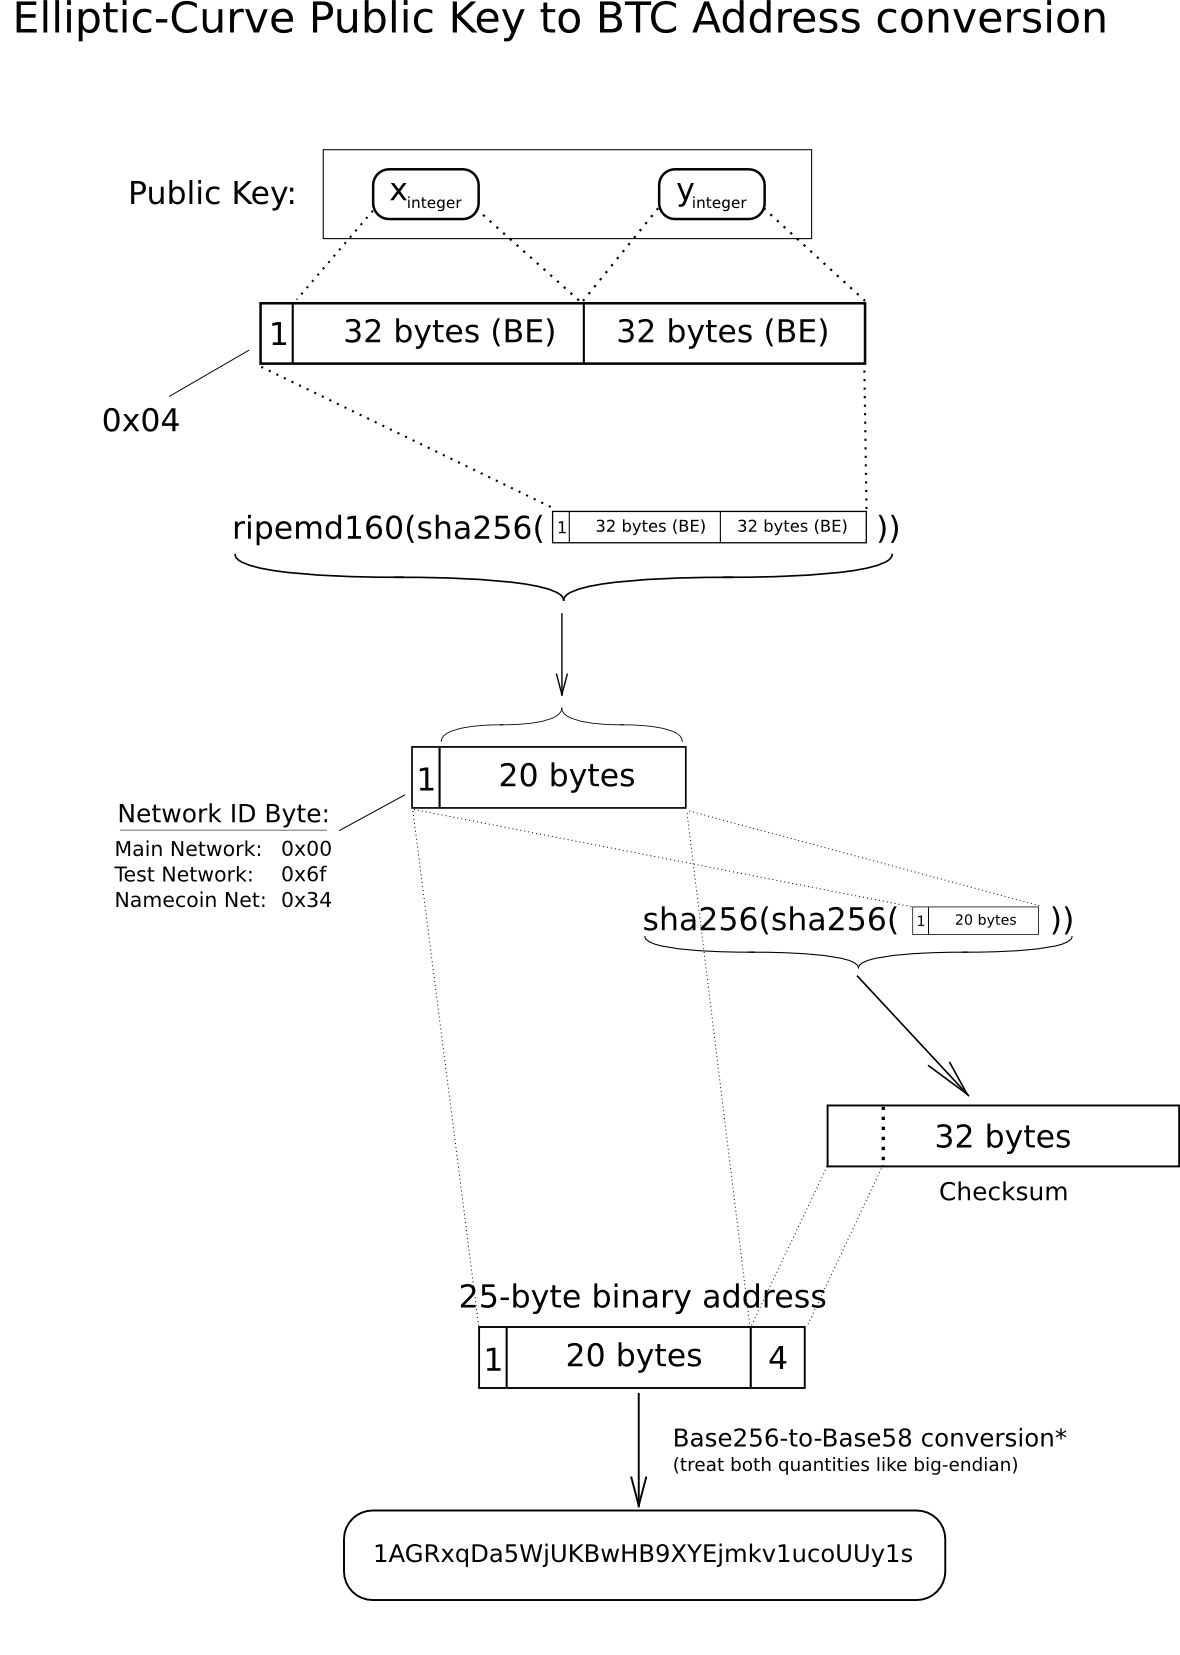
\includegraphics[width=0.7\textwidth]{figs/PubKeyToAddr.png}
   
   \label{fig:PubKeyToAddr}
\end{figure}
%A private key can't be determined by knowing the public key, and it is safe for the public key to be known by anyone.

An analogy of a postal box can be used to explain a Bitcoin address. The public address is like a post box. Anyone can deposit something into the box without having access to the key of the box. They only need to know the box number to make the deposit. To retrieve or spend whatever is in the box, they need the key. Therefore, the private key is like the key to the post box. Only the person with the key can open the box and retrieve the content. One important difference to a normal postal box is that the postal box is completely transparent, meaning anyone can see exactly what is in the box.

\subsection{How Bitcoins Are Stored}
\label{sbs:bitcoin_stored}

Bitcoin is ``stored'' using a public ledger called the blockchain. Effectively, every single successful Bitcoin transaction is stored in this public ledger, and every user that runs a full Bitcoin node has an identical copy of the blockchain. The authenticity of the blockchain is managed by using consensus on the network and using hashing alogrithms. Bitcoin transactions are bundled into blocks, and the entire block is hashed. This block is hashed with the hash of the previous block as input, and so forth in the chain until the first block is reached. Every block's hash is the hash of the entire chain behind it as can be seen in figure \ref{fig:Blockchain}. This means that nothing can be changed in the chain, since it will change the entire hash after the change.

Since the entire ledger of Bitcoin transactions is publicly available, it is possible to calculate the balance of any address at any given time. To store a Bitcoin wallet, only the private key of the wallet is required. A wallet is not a file containing Bitcoin. The ownership of the Bitcoin is recorded in the Blockchain. Even though the public address is derived from the private key, a server usually stores the public address as well, since it will be inefficient to calculate it everytime a lookup is needed. The fact that we only need to store these two values in order to have access to the Bitcoin is the most relevant part of how Bitcoin works for our purposes. It allows a developer to simply store these two simple values securely, without having to keep track of complex databases locally.

\begin{figure}
  \centering
  	\caption{Simplified representation of Bitcoin blockchain. Adapted from \cite{Nakamoto2008}.} 
    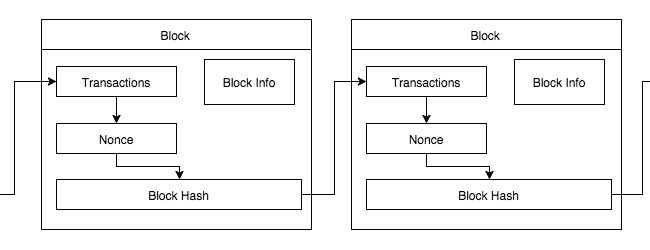
\includegraphics[width=\textwidth]{figs/Blockchain.png}
   
   \label{fig:Blockchain}
\end{figure}

\subsection{How a Bitcoin Transaction Works}

Since the blockchain is a public ledger of all transactions, it is a crucial part of making a new transaction. Every transaction has inputs and outputs. An input in a transaction is an output from a previous transaction to form a transaction chain. This output can then be used as a new input for a new transaction as can be seen in figure \ref{fig:transactions}.

 When looking at an address on the blockchain, we can determine which of the outputs of its transactions are not spent yet. They are called unspent outputs. These outputs can be cryptographically verified to belong to a specific address and can be used as inputs in a new transaction. The transaction then specifies new outputs to send Bitcoin to. To receive ``change'' in a Bitcoin transaction, the change amount must be specified to the address that the payer chose. The change address can be a new address owned by the payer, or the same address that the payment came from.

The difference between the sum of the inputs and outputs of a transaction is the transaction fee that is claimed by users that verify transactions. This is called mining and is discussed in section \ref{sbs:bitcoin_mining}.

\begin{figure}
  \centering
  	\caption{Example of Bitcoin transactions demonstrating the relationship between inputs and outputs\cite{bitcoinOrg}.} 
    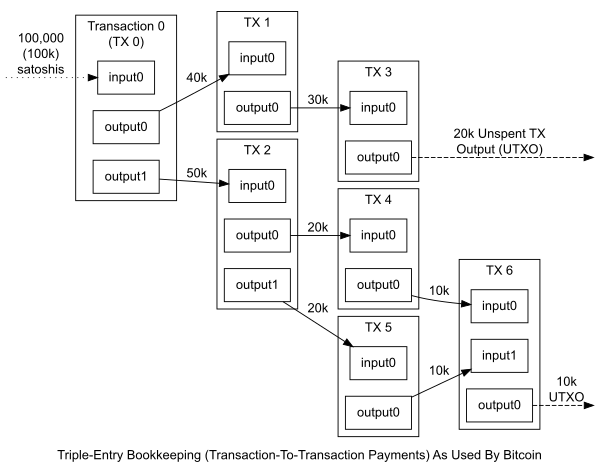
\includegraphics[width=0.9\textwidth]{figs/en-transaction-propagation.png}
   
   \label{fig:transactions}
\end{figure}

\subsection{Bitcoin Mining}
\label{sbs:bitcoin_mining}

Bitcoin mining is the process of bundling transactions together to form a block. As mentioned in \ref{sbs:bitcoin_stored}, every block has a hash that is in effect the hash of the entire chain. For a block to be valid, this hash has to satisfy the condition of leading with a certain number of zeros. Its only purpose is to be difficult to do, so that a lot of work is required to do so. The only way of doing this is using a brute force method. Therefore, more computation power increases the probability of finding a block that satisfies the zeros criteria. 

The number of zeros required is called the ``difficulty'', since more zeroes makes it more difficult to find a valid block. The difficulty dynamically updated by the Bitcoin network to ensure that the average time for finding such a block is 10 minutes.

When a transaction is mined into the most recent block, it has 1 confirmation. The longer the chain becomes after this block, the more confirmations it has and the transaction can with higher trust be regarded as final. Valid transactions that are published to the Bitcoin network are stored in each nodes memory pool (mempool) until they are mined into a block or discarded \cite{bitcoinOrg}. These transactions have 0 confirmations. 

For example, a transaction with only one confirmation can still be rejected if a successful double spend attack is done. With more confirmations, the probability of a double spend attack lowers exponentially \cite{Nakamoto2008}. With very small payments, it is not  not required to have many confirmations to accept a payment. It is worth the risk of accepting a payment with 0 confirmations, since it is not worth the effort to try and do a double spend on such a small transaction.

\section{REST}
\label{rest}

Representational State Transfer (REST) is a Web architecture introduced in 2000 by Roy Fielding \cite{Fielding2000}. REST uses a client-server model to transfer data to and from the server. The interaction between the client and server is designed to be stateless. Therefore, every request to the server and every answer must contain all the information to complete the request. The stateless design induces visibility, reliability and scalability according to Fielding\cite{Fielding2000}.

\begin{figure}
  \centering
  	\caption{Client-server Model of REST architecture\cite{Fielding2000}.} 
    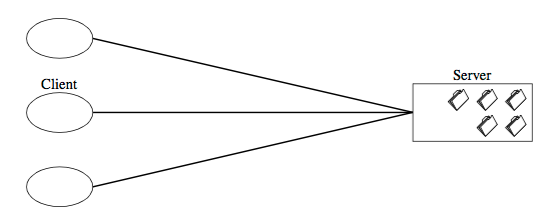
\includegraphics[width=0.8\textwidth]{figs/rest_client_server.png}
   
   \label{fig:rest_client_server}
\end{figure}

REST uses HTTP methods explicitly \cite{IBM} to transfer resources to and from the server as described in table \ref{tbl:rest_methods}. Since standard HTTP methods are used, Web servers do not need to use specialised protocols to use a REST architecture. Furthermore, the REST service can be built using any backend webserver software that is capable of receiving the HTTP methods from table \ref{tbl:rest_methods}, has a scripting language and preferably some sort of storage like a database.

\begin{table}
	\begin{center}
		\caption{HTTP Methods used in the REST Architecture\cite{IBM}.} 
		\begin{tabular}	{ | c | c |}
		\hline
		\textbf{HTTP Method} & \textbf{Usage In REST} \\ \hline
		POST & Create resource on server \\ \hline
		GET & Retrieve resource from server \\ \hline
		PUT & Change or update resource \\ \hline
		DELETE & Remove resource \\ \hline
		
	 
	   % \label{fig:htaccess_file}
		\end{tabular}
		
		\label{tbl:rest_methods}
	\end{center}
\end{table}

REST uses URIs (Uniform Resource Identifiers) to distinguish method calls that are being made. The URI contains the names of specific resource that is required in a hierarchical structure. For example, the URI \\``http://www.myservice.org/discussion/topics/{topic}'' would call the service at myservice.org with a specific topic in the topics category under the discussion category \cite{IBM}. The curly brackets indicate a variable. Therefore, ``{topic}'' would be replaced with something like ``sport''. These URIs usually do not contain file extensions, like ``.php'', to be able to change the backend scripting language without changing the URIs. 

\section{Gamebooks}

Gamebooks, Interactive Fiction and Choose Your Own Adventure are terms used for stories told in a non-linear way where the user is presented with choices that influence the flow and outcome of the story. The Choose Your Own Adventure brand of books was first published in 1979 after an author called Ed Packard aproached a small publisher in 1976 with a gamebook manuscript \cite{cyoa}.

In a typical gamebook, the reader is given choices that are made by going to the page number indicated by the choice. For example, a reader can be given a choice of going through one of two doors. The choice can tell the reader to go to page 55 to go through the first door or to page 56 to go through the second door. If a gamebook is read only once, many pages of the book will not be read.

According to cyoa.com, gamebooks appeal to reluctant readers do to the interactive nature of gamebooks \cite{cyoa}. 

Gamebooks are also available electronically. A company called Choice of Games \cite{CoG} is an example of an electronic gamebook publisher. Their gamebooks are available on a browser or on standalone mobile apps. They created a scripting language called ``ChoiceScript'' to allow authors to write gamebooks in an easy and intuitive way. 

Since a gamebook is a piece of text with options as links, any website can easily be made into a gamebook. A website called Create Your Own Story \cite{editthis} uses a MediaWiki \cite{mediawiki} framework to write gamebooks that anyone can contribute to.  

\begin{figure}
  \centering
  	\caption{Example of one of the earliest Choose Your Own Adventure books \cite{cyoa}.} 
    
\includegraphics[width=0.4\textwidth]{figs/cyoa.jpg}
   
   \label{fig:cyoa_book}
\end{figure}

